\section{Penelitian Terkait}

Pada sub-bab ini,  dibahas beberapa penelitian yang telah dilakukan terhadap penggunaan metode PEFT pada \textit{pre-trained model}.

\subsection{\textit{Unified View of Parameter-Efficient Transfer Learning}}

\textit{Unified Parameter Transfer Learning} merupakan upaya untuk menggabungkan beberapa metode PEFT menjadi satu kesatuan \textit{framework} \parencite{uvpl}. Dalam \textit{transfer learning}, ide utamanya adalah mengambil \textit{pre-trained model} dan menyesuaikannya untuk tugas yang berbeda. Namun, ada banyak cara untuk melakukan adaptasi ini, dan setiap metode memiliki karakteristiknya masing-masing. Beberapa teknik mungkin fokus pada penambahan lapisan adaptasi, sementara yang lain mungkin memprioritaskan modifikasi parameter tertentu dalam model.

Metode PEFT lain telah berhasil mengubah atau menambahkan sedikit parameter untuk mendapatkan kinerja yang setara dengan \textit{fine-tuning} , tetapi hubungan antara metode tersebut tidak dimengerti secara baik \parencite{uvpl}. Selain itu, dicari juga elemen desain pada metode ini yang menjadi aspek penting pada kesuksesan metode terkait. \citeauthor{uvpl} pada penelitiannya ini, mencari hubungan antara tiap metode ini dengan mengupas arsitektur dari setiap metode terkait. Metode yang digunakan pada penelitian yang dilakukan oleh \citeauthor{uvpl} adalah LoRA, \textit{prefix-tuning}, dan \textit{adapter}.

\begin{figure}[ht]
    \centering
    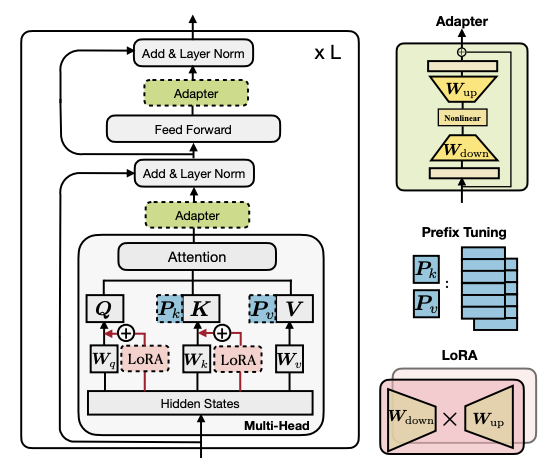
\includegraphics[width=0.8\textwidth]{chapter-2/uvpl.png}
    \caption{Arsitektur \textit{Unified View of Parameter-Efficient Transfer Learning} \parencite{uvpl}}
    \label{fig:uvpl}
\end{figure}

% TODO: tambahin secara jelas gimana tiap metode ini jadi satu dan hubungannya gimana
Arsitektur yang diajukan oleh \citeauthor{uvpl} pada penelitiannya dapat dilihat pada Gambar \ref{fig:uvpl}. Arsitektur tersebut menggabungan metode yang disebutkan sebelumnya pada model berbasis \textit{transformer}. 

\subsection{\textit{Parameter-Efficient Fine-Tuning of Large-Scale
Pre-Trained Language Models}}

Penelitian yang dilakukan oleh \citeauthor{peft_on_plm} membandingkan secara komprehensif terkait metode \textit{transfer-learning} yang efisien secara parameter pada \textit{pre-trained model}. Metode ini disebut sebagai \textit{delta-tuning} pada penelitian tersebut, dengan kata 'delta' muncul dari notasi matematika yang merepresentasikan perubahan \parencite{peft_on_plm}. Metode \textit{delta-tuning} yang digunakan adalah \textit{prompt-tuning} (PT), \textit{prefix-tuning} (PF), LoRA (LR), dan \textit{adapter} (AP). \textit{Delta-tuning} tersebut  dibandingkan dengan \textit{fine-tuning} (FT) .

Eksperimen yang dilakukan pada penelitian tersebut dilakukan pada model T5 dengan konfigurasi BASE dan LARGE. Evaluasi metode \textit{delta-tuning} pada model T5 dilakukan pada 100 tugas pemrosesan bahasa alami yang diambil dari \textit{dataset} Huggingface. Tugas yang dipilih termasuk \textit{text classification}, \textit{question answering}, dan \textit{generation}.

Berdasarkan hasil yang didapatkan pada eksperimen tersebut, metode \textit{delta-tuning} dengan pengurangan jumlah parameter yang dilatih dibandingkan dengan \textit{fine-tuning} memberikan hasil yang hampir setara pada sebagian besar tugas. Metode \textit{prefix-tuning}, LoRA, dan \textit{adapter} secara kinerja hampir mirip antara satu sama lain. Bahkan, metode \textit{delta-tuning} pada sebagian tugas mampu memberikan hasil yang dominan dibanding \textit{fine-tuning}. Secara keseluruhan, kinerja pada setiap metode dapat diurutkan sebagai berikut.

\begin{enumerate}
    \item \textit{Fine-Tuning} (FT)
    \item \textit{Low-Rank Adaptation} (LoRA)
    \item \textit{Adapter Tuning} (AP)
    \item \textit{Prefix Tuning} (PF)
    \item \textit{Prompt Tuning} (PT)
\end{enumerate}

Selain itu, dilakukan juga eksperimen terkait analisis pada efisiensi dari tiap metode. Eksperimen ini mengeksplorasi penggunaan efisiensi memori GPU pada metode \textit{delta-tuning} dan FT pada model T5 dengan konfigurasi BASE, LARGE, dan XL. Metode \textit{delta-tuning} yang digunakan adalah LoRA (LR), dan \textit{adapter} (AP), dan BitFit (BF). Berdasarkan Gambar \ref{fig:peft_on_plm_memory}, penggunaan memori pada setiap metode \textit{delta-tuning} berkurang dibandingkan dengan \textit{fine-tuning}. Hasil ini menunjukkan bahwa \textit{delta-tuning} mengurangi penggunaan memori GPU dengan mengurangi kebutuhan komputasi gradien untuk mengubah parameter.

\begin{figure}[ht]
    \centering
    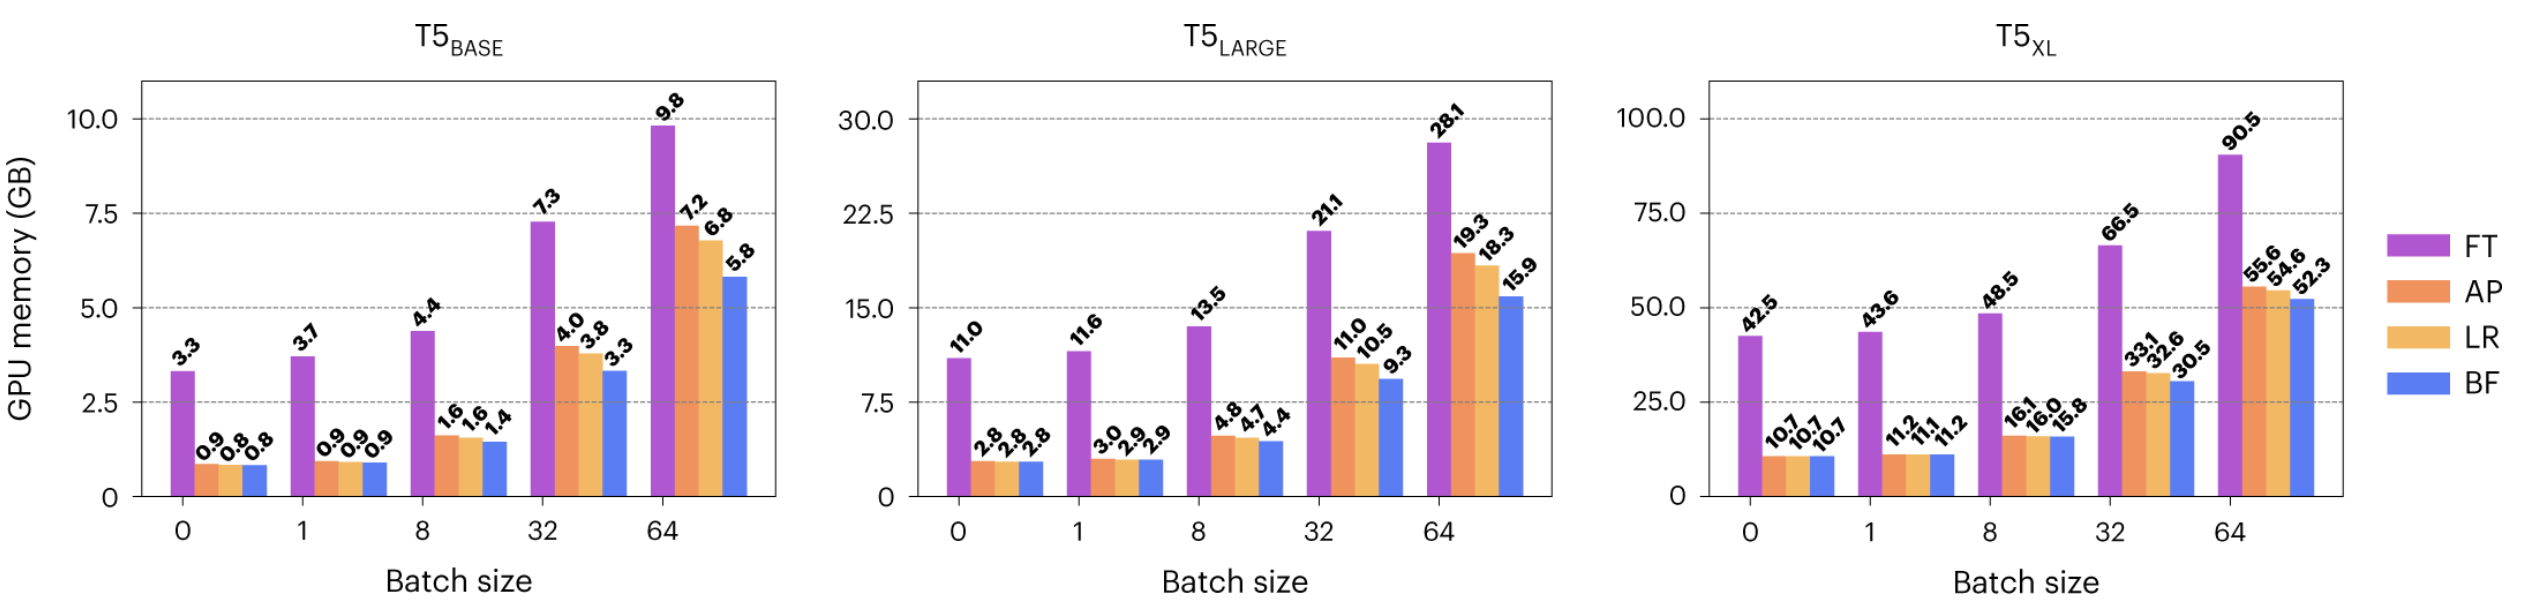
\includegraphics[width=1\textwidth]{chapter-2/peft_on_plm_memory.png}
    \caption{Perbandingan Efisiensi Memori \parencite{peft_on_plm}}
    \label{fig:peft_on_plm_memory}
\end{figure}
